\section{Motivating Examples}
\label{sec:motiv}

We begin our motivation for a tool such as \app by providing several misconfiguration examples, and showing how do we address them. All these examples are extracted from real-world reports%
~\cite{yin11anempirical, configdataset}. When writing configuration files, the user usually takes already existing files and modifies them. If the original file is already corrupted, the errors are propagated further. However, even if the original file is correct, changing the file by a non-expert user can easily result in errors.


\subsection{Ordering Errors}

When configuring PHP to run with the Apache HTTP Server the user writes, among others, the following lines:\\
 \texttt{
 \hspace*{3em}extension = mysql.so\\
 \hspace*{3em}...\\
 \hspace*{3em}extension = recode.so}\\
This file caused that the Apache server could not start due to 
the segmentation fault error. Running \app on this file returns\\
 \texttt{
  one line output from our tool that indicates that things should be reordered}\\
Indeed, this was the source of the error. When using PHP in Apache, the
extension ``mysql.so'' depends on ``recode.so'' and the relative ordering 
of two of them is crucial. The user is informed that ``recode.so'' should appear before ``mysql.so''.


\begin{figure}[t] \centering
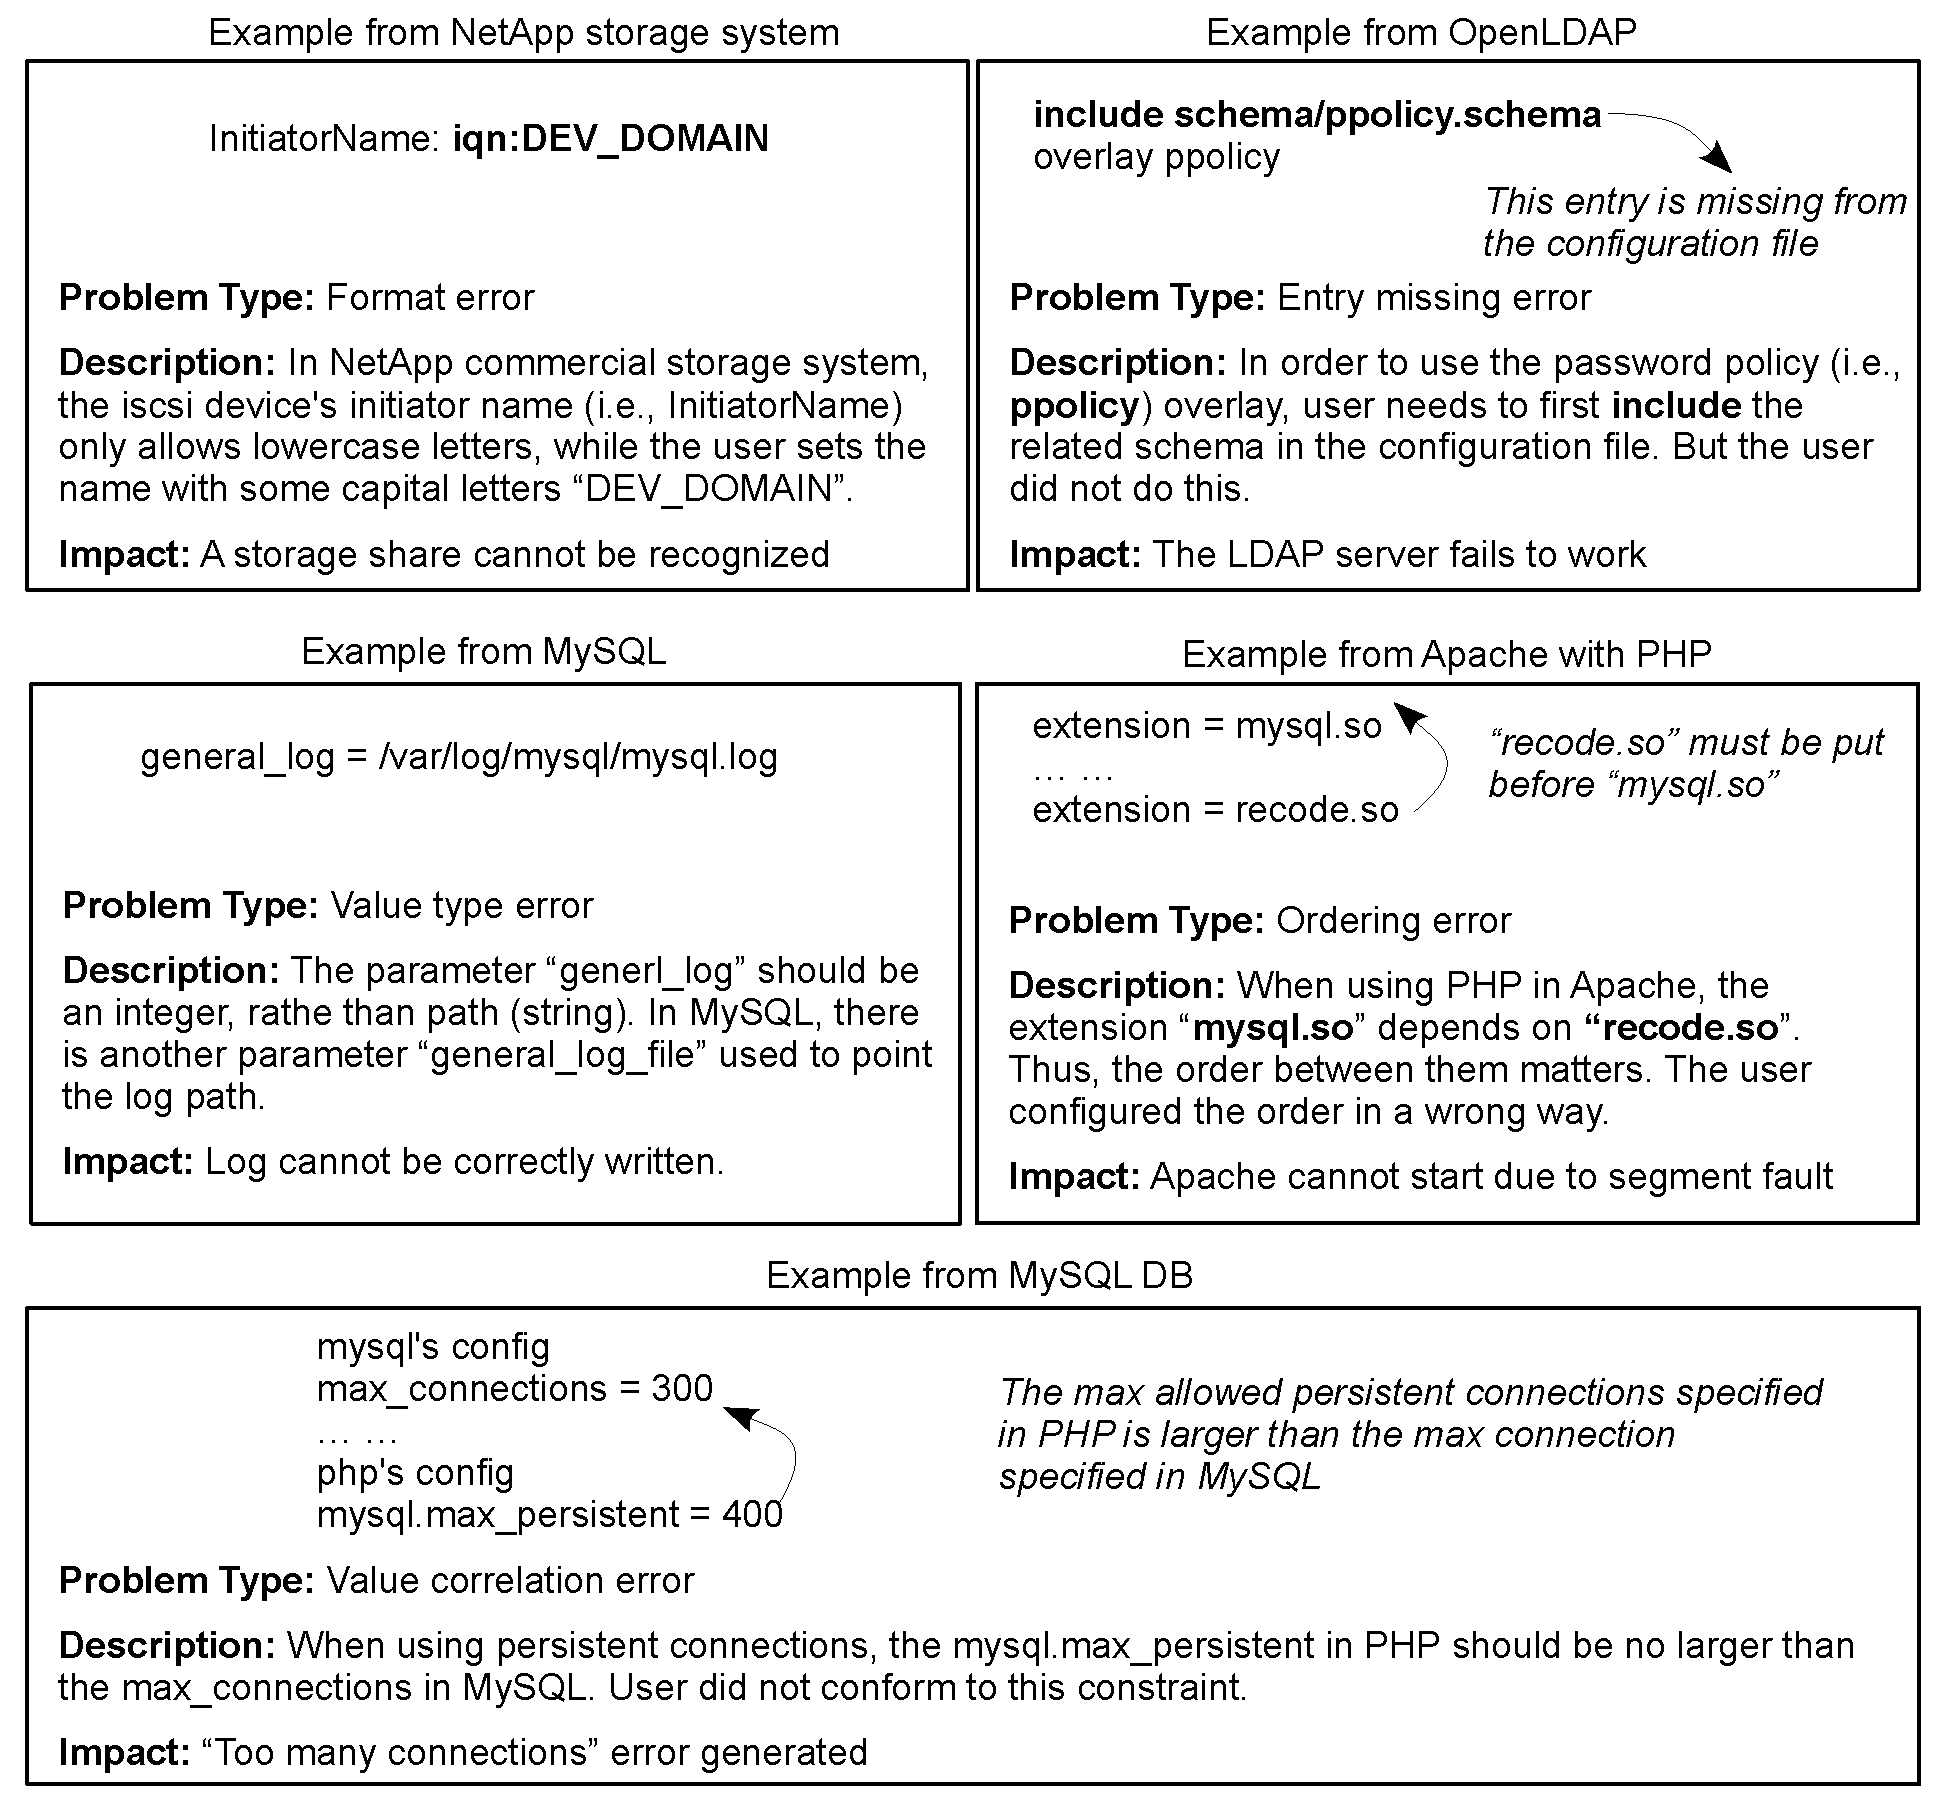
\includegraphics[width=0.98\textwidth]{figs/example}
\caption{Motivating examples. Our target configuration errors are
  classified into five groups. The five examples here correspond to
  these groups, respectively.}
\label{fig-example}
\end{figure}

Fig.~\ref{fig-example} presents misconfiguration examples in real-world
that we aim to address. All the examples are extracted from
misconfiguration issues reported in real-world efforts%
~\cite{yin11anempirical, configdataset}.
We classify our target configuration errors
into five groups: 1) format error; 2) entry missing error; 3) value type
error; 4) ordering error; and 5) value correlation error.
The five examples in Fig.~\ref{fig-example} correspond to the above five
groups, respectively.

 
